\documentclass[10pt]{article}
\usepackage{amsmath}
\usepackage{amsfonts}
\usepackage[utf8]{inputenc}
\usepackage[margin=0.5in]{geometry}
\usepackage{graphicx}

\usepackage[T1]{fontenc}
\usepackage[scaled]{beramono}
\renewcommand*\familydefault{\ttdefault}
\usepackage{listings}

\lstset{
  language=Python,
  showstringspaces=false,
  formfeed=\newpage,
  tabsize=4,
  commentstyle=\itshape,
  basicstyle=\ttfamily,
  morekeywords={models, lambda, forms}
}

\newcommand{\code}[2]{
%   \hrulefill
  \subsection*{#1}
  \lstinputlisting{#2}
  \vspace{2em}
}

% Title Page
\title{CBE 502 - HW7 - Finite Elements}
\author{Tom Bertalan}


\begin{document}
\maketitle

\tableofcontents

\listoffigures

\section{Analytical Solution by Green's Function}
\label{sec:green}

\subsection{Problem}

\begin{equation}
\label{eqn:problem}
\begin{split}
 L[u(x)] &= -f(x) \\
L[u(x)] &=  \frac{\partial^2 u}{\partial x^2} \\
-f(x) &= A \sin (\omega x) + m x
\end{split}
\end{equation}

Boundary conditions:

\begin{equation}
 \begin{split}
    \left. u(x) \right| _{x=0} &= 1 \\
    \left. \frac{\partial u(x)}{\partial x}\right|_{x=1} &= \epsilon
 \end{split}
\end{equation}

Constants:

\begin{equation}
\label{eqn:constants}
 \begin{split}
    A = 18.0 \\
    \omega = 10.0 \\
    m = 4.0 \\
    \epsilon = 0.5
 \end{split}
\end{equation}


Change of variables, to create homogeneous boundary conditions:

\begin{equation}
\label{eqn:changeofvars}
 \begin{split}
  v = u + a x + b \\
  v' = u' + a \\
 \end{split}
\end{equation}

To make the new boundary conditions homogeneous, choose $b=-1$ and $a=-\epsilon$.

$$
-f(x) = L[u] = \frac{\partial^2 v}{\partial x^2} + 0 + 0 = L[v]
$$

That is, the problem does not change with the change-of-variables, only the boundary conditions.

\subsection{Properties of the Green's Function}
$$\quad$$
$G(x,t)$ satisfies the homogeneous problem (that is, $G''(x,t) = 0$):
    
\begin{equation}
G(x,t) = 
 \left\{ \begin{matrix}
    C_{1,1} x + C_{1,2}, \quad 0 \le x \le t \\ 
    C_{2,1} x + C_{2,2}, \quad t \le x \le 1
    \end{matrix} \right\}
    =
    \left\{ \begin{matrix}
    C_{2,1} x + C_{2,2}, \quad 0 \le t \le x \\ 
    C_{1,1} x + C_{1,2}, \quad x \le t \le 1
    \end{matrix} \right\} 
\end{equation}

$G(x,t)$ satisfies homogeneous boundary conditions:
    
\begin{equation}
 \begin{split}
  G(0,t) = 0 = C_{1,1} \cdot 0 + C_{1,2}  &\xrightarrow{ } C_{1,2} = 0 \\
  G'(0,t) = 0 = C_{2,1} \quad \quad  &\xrightarrow{ } C_{2,1} = 0
 \end{split}
\end{equation}

$G(x,t)$ is piecewise, but fully continuous:
\begin{equation}
\label{eqn:continuous}
\begin{split}
    \lim _{ x \rightarrow t^- }{G(x,t)} &= \lim _{ x \rightarrow t^+ }{G(x,t)} \\
    C_{1,1}(t)\cdot t &= C_{2,2}(t)
\end{split}
\end{equation}

$G'(x,t)$ has a jump discontinuity of $1/p(x)$, where $p(x)=1$ is taken from the standard from of the second-order operator $L[u(x)]$:
    
\begin{equation}
\label{eqn:jump}
 \begin{split}
  \left. \frac{\partial G}{\partial x} \right| _{t^+} - \left. \frac{\partial G}{\partial x} \right| _{t^-} &= 1 \\
  0 - C_{1,1}(t) &= 1
 \end{split}
\end{equation}

From (\ref{eqn:continuous}) and (\ref{eqn:jump}), we find that $C_{1,1}=-1$ and $C_{2,2}(t)=-t$. So, the completed Green's function for this operator is:
\begin{equation}
\label{eqn:green}
G(x,t) = 
 \left\{ \begin{matrix}
    -x, \quad 0 \le x \le t \\ 
    -t, \quad t \le x \le 1
    \end{matrix} \right\}
    =
    \left\{ \begin{matrix}
    -t, \quad 0 \le t \le x \\ 
    -x, \quad x \le t \le 1
    \end{matrix} \right\} 
\end{equation}

The solution (with the change-of-variables) is then given by integrating the product of the Green's function and the forcing function:
\begin{equation}
\label{eqn:v(x)}
 \begin{split}
  v(x) &= \int_{x=a}^{x=b}{-f(t) \quad G(x,t) \quad dt} \\
  &= \int_{0}^{x}{-f(t)(-t)dt} + \int_{x}^{1}{-f(t)(-x)dt} \\
  &= \frac{m \omega^2 x (-3 + x^2) + 6 A \omega x \cos(\omega) - 
 6 A \sin(\omega x)}{6 \omega^2}
 \end{split}
\end{equation}

Check:
    
\begin{equation}
 \begin{split}
  \left. v(x) \right|_{x=0} &= 0 \quad \checkmark \\
  \left. \frac{\partial v(x)}{\partial x} \right|_{x=1} &= 0 \quad \checkmark \\
  \frac{\partial^2 v(x)}{\partial x^2} - (-f(x)) &= 0 \quad \checkmark
 \end{split}
\end{equation}


The true solution can be obtained by inverting the change-of-variables:
    
\begin{equation}
\label{eqn:u(x)}
 \begin{split}
  u(x) &= v(x) + x/2 + 1 \\
  &= 1 + \epsilon x - \frac{m x}{2} + \frac{m x^3}{6} + \frac{A x \cos(\omega)}{\omega} -
   \frac{A \sin(\omega x)}{\omega^2}
 \end{split}
\end{equation}

Check, 

\begin{equation}
 \begin{split}
  \left. u(x) \right|_{x=0} &= 1 \quad \checkmark \\
  \left. \frac{\partial u(x)}{\partial x} \right|_{x=1} &= \epsilon \quad \checkmark \\
  \frac{\partial^2 u(x)}{\partial x^2} - (-f(x)) &= 0 \quad \checkmark
 \end{split}
\end{equation}
    
\section{Finite Element Solution}
\label{sec:FE_work}

\section{Results}
\label{sec:results}

\begin{figure}[ht]
 \centering
 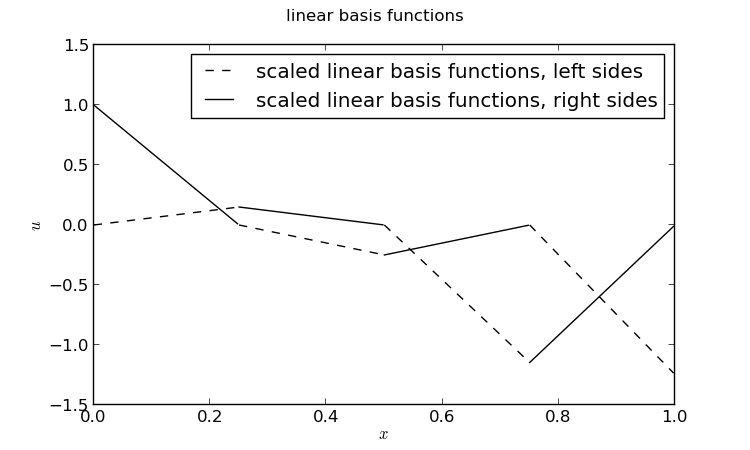
\includegraphics[width=\columnwidth,keepaspectratio=true]{./hw7-basis_functions-N5.png}
 % hw7-basis_functions-N5.png: 1000x600 pixel, 100dpi, 25.40x15.24 cm, bb=0 0 720 432
 \caption{Five basis functions.}
 \label{fig:N5}
\end{figure}

\begin{figure}[ht]
 \centering
 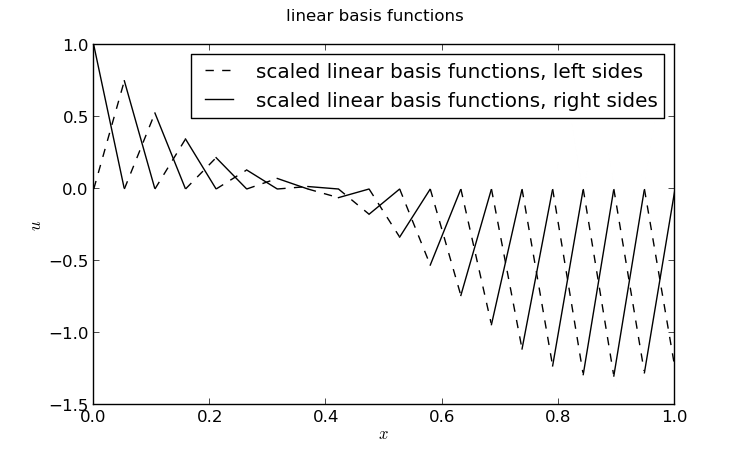
\includegraphics[width=\columnwidth,keepaspectratio=true]{./hw7-basis_functions-N20.png}
 % hw7-basis_functions-N20.png: 1000x600 pixel, 100dpi, 25.40x15.24 cm, bb=0 0 720 432
 \caption{Twenty basis functions.}
 \label{fig:N20}
\end{figure}

\begin{figure}[ht]
 \centering
 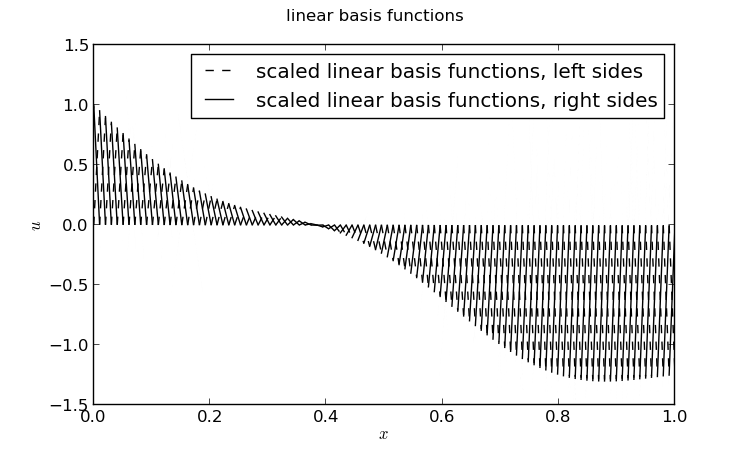
\includegraphics[width=\columnwidth,keepaspectratio=true]{./hw7-basis_functions-N100.png}
 % hw7-basis_functions-N100.png: 1000x600 pixel, 100dpi, 25.40x15.24 cm, bb=0 0 720 432
 \caption{One hundred basis functions.}
 \label{fig:N100}
\end{figure}

\begin{figure}[ht]
 \centering
 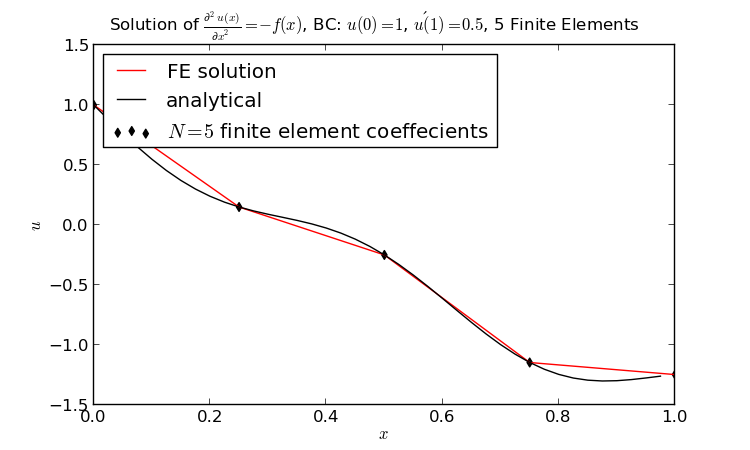
\includegraphics[width=\columnwidth,keepaspectratio=true]{./hw7-solution_and_forcing-N5.png}
 % hw7-solution_and_forcing-N5.png: 1000x600 pixel, 100dpi, 25.40x15.24 cm, bb=0 0 720 432
 \caption{Solution and forcing, 5 basis functions.}
 \label{fig:sf5}
\end{figure}


\begin{figure}[ht]
 \centering
 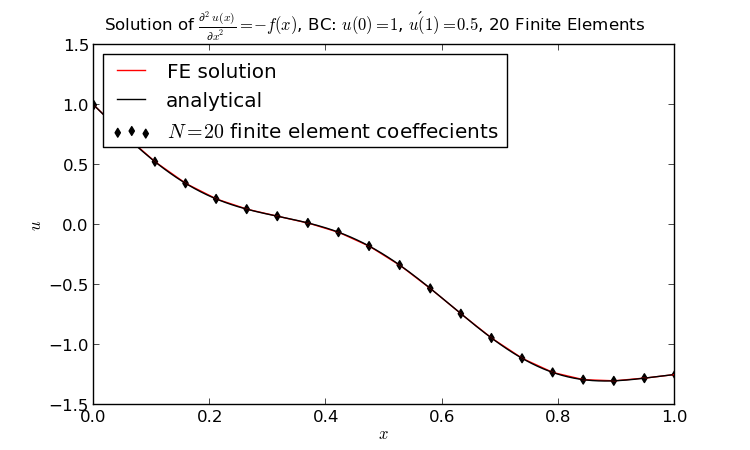
\includegraphics[width=\columnwidth,keepaspectratio=true]{./hw7-solution_and_forcing-N20.png}
 % hw7-solution_and_forcing-N5.png: 1000x600 pixel, 100dpi, 25.40x15.24 cm, bb=0 0 720 432
 \caption{Solution and forcing, 20 basis functions.}
 \label{fig:sf20}
\end{figure}


\begin{figure}[ht]
 \centering
 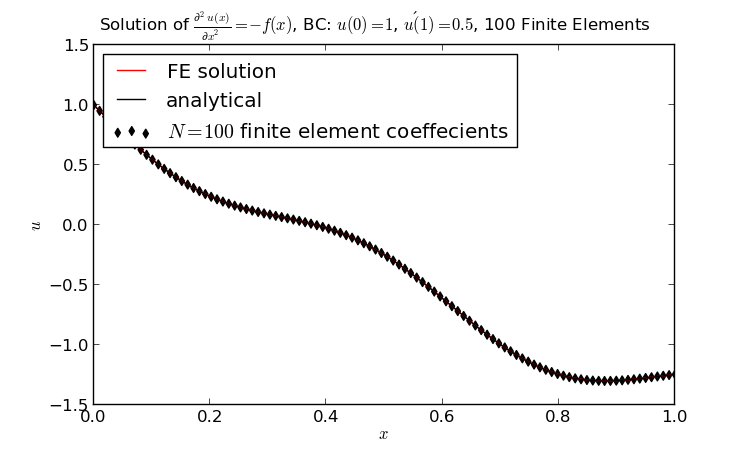
\includegraphics[width=\columnwidth,keepaspectratio=true]{./hw7-solution_and_forcing-N100.png}
 % hw7-solution_and_forcing-N5.png: 1000x600 pixel, 100dpi, 25.40x15.24 cm, bb=0 0 720 432
 \caption{Solution and forcing, 100 basis functions.}
 \label{fig:sf100}
\end{figure}

\begin{figure}[ht]
 \centering
 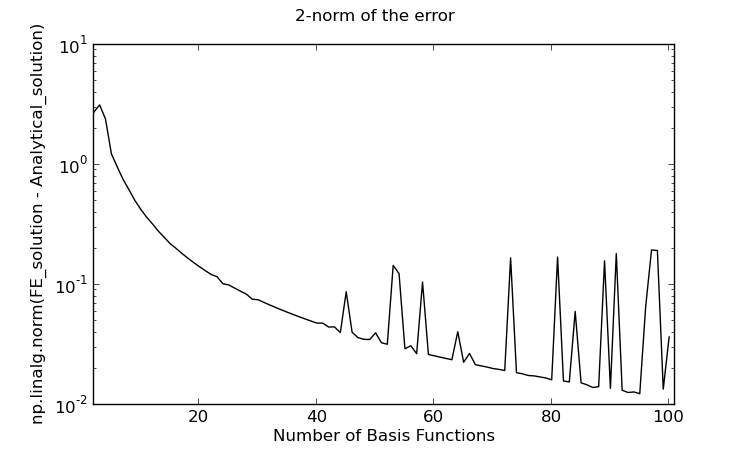
\includegraphics[width=\columnwidth,keepaspectratio=true]{./hw7-error_rate.png}
 % hw7-error_rate.png: 1000x600 pixel, 100dpi, 25.40x15.24 cm, bb=0 0 720 432
 \caption{Rate of error reduction with increasing number of basis functions (decreasing discretization distance).}
 \label{fig:errorrate}
\end{figure}

\clearpage

\section{Code}

\code{hw7.py}{hw7.py}

\end{document}          
